%
% loesung_rechenbsp.tex
%
% (c) 2024 Flurin Brechbühler
%
\begin{figure}
    \centering
    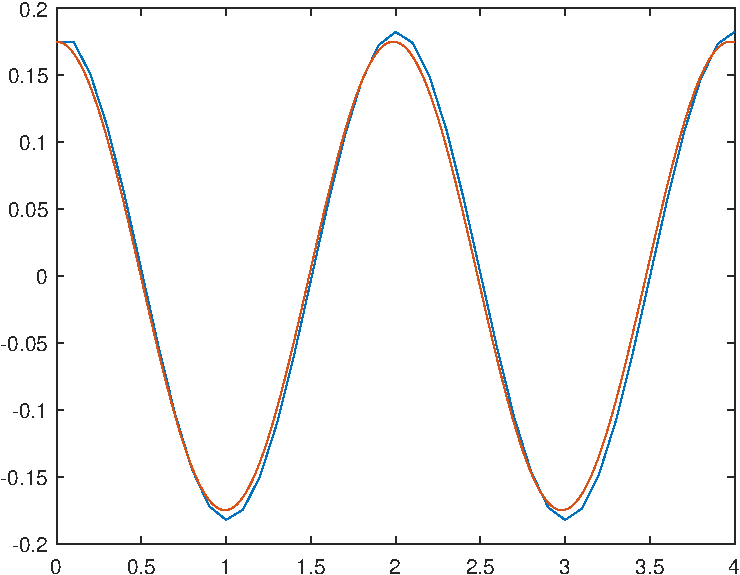
\includegraphics[width=\textwidth]{papers/fem/images/loesung_rechenbsp.pdf}
    \caption{Die mit der FEM erhaltene Lösung in Blau und die analytische Lösung in Rot.}
    \label{fem:rechenbsp:loesung}
    \end{figure}
    